State our focus of COO and MTX formats (but we study only MTX format in these experiments).
We appropriately handle the header of the file format.

The mmap interface is faster than the traditional read/write because it avoids the system call overhead and copies between the kernel and user space. However, I/O with mmap is synchronous and has more complex error handling. For instance, on a disk full a write would return with an error code, while mmap-based I/O would require handling a signal \cite{enberg2022transcending}.

In contrast, Direct I/O (DIO) allows applications to use the same read and write system calls while bypassing the page cache. However the buffer management and caching is performed in user space \cite{enberg2022transcending}.




\subsection{Reading Edgelist from text file}

\textbf{approach-read-stream-plain}:

In this approach, we use C++'s ifstream to open the file, and read the edges line by line. If the graph is unweighted, we simply read the source and target integers as sizet into source and target arrays that are pre-allocated based on information in the header of the file (rows, cols, size). If the graph is weighted, we also read the weights as 32-bit floating point numbers into another preallocated array. We do this seqeuntiall as the stream sare inherently sequential. Is this buffered, please check? Why are C++'s stream slow? virtual calls?

\textbf{approach-read-stream-strtoull}

In this approach, we again use C++'s ifstream - but use string to number conversion methods strtoull and strtod to perform number parsing in parallel. For this, we first read a chunk of 128K lines from the file sequentially from ifstream using getline, and then parse each line using multiple threads in parallel (with OpenMP's dynamic scheduling with chunk size of 1024, which we observe performs well). Once the edges are parsed (source, target, weight), we store them separately in per thread edge-lists to avoid contention issue into a shared data structure. With 64 threads, this approach provided a speed improvement of XX, compared to approach-read-stream-plain.

\textbf{approach-read-fscanf-plain}

This appraoch is ismilar to the approach mentioned above, but we use fgets on a file handle, instead of ifstream >> operator, and use sscanf to parse the edges (source, target, weight - if weighted). This approach can be performed in parallel. With 64 threads, this approach provede a speedup of X wrt to X.

\textbf{approach-read-fscanf-strtoull}

This approach is similar to the approach above, but use use strtoull and strtod instead of sscanf. This is faster due to the absence of having to parse a format string. With 64 threads, this approach provide a speedu pof X over X.

\textbf{approach-read-mmap-sscanf}

It is possible to read chunks of a file using fread, and process them in parallel. However, such reads can only be performed sequentially, requires special logic and additional buffers to keep track of partial lines and both ends of a chunk, requires synchronization between threads, and data loaded into memory needs to be swapped out to disk in case of low memory. This is in contrast to memory mapped files, which use mmap, to which map files to the mmroy space b yusing the paging mechanism  -provided my all modern processors supporting virtual memory. In fact it is the paging mechanism. Here, a initial mapping of memory address range to the file is ceated by the kernel. When a thread access a memory that is not loaded from disk, a page fault occurs and the page (4K) is loaded into memory and the page table is updated. The kernel can unload the page instantly if the system is low on memory (if no writes have been made to the page). With memory mapping, extremenly large file can be easily mapped to memory, thanks to 64-bit memory addresses, and conviniently processed by threads. In additiona requenct to load pages can be made in parallel by multiple threads. This, in addition to a number of other reasons, makes mmap an attractive choice for IO.
[Maybe move this to preliminaries]

We can also use mmap to allocate memory for the current process. The kernel ensures that the allocated meory is zero-filled upon use.

madive can be used to instruct the kernel about the page access pattern in order to optimize loading of pages. We observe that an madvaise of eiki gives good performance. We also observe that using a chunk size of 256K gives goood parallel performance with memory mapped files. This is what is use in the rest of the report.
(We use file bytes sum experiment for this - take some details from there).

For process edges in parallel using multiples thread (64), we assign chuncks of size 256K to each thread. Each thread works as follows. ItEach thread processes the chunk assign to it sequentilly. First, if the chunk has partial lines and the begin and at the end of the chunk, it re posistion the chunk such that the chunk had no partial lines (use BLOCK term, not chunk). To do this, it skips the partial line at the beign of the chunk, and the includes partial line from the end of the chunk. Then it procees the lines (edges) sequentially.

To process the edges, we use sscanf, strttoull/strtod, and a custom number parsing function for both whole numbers and floats. The last approach gives us the best performance as shown in figure X. We also attempt using custom SIMD sintructions to parse integers in parallel along with vzeroupper to cleasr sse/avx register to avoid performance peonalty. Unfortunatele, this provied us with no additional improve ment in performance. Finally we decrement a BASE values from the parse number to make the vertex-ids zero-based. The relative runtime is hsown in Figure X. This needs to be done appropriately, otherwise there can be a large performance penaltl. Using weighted flag as a template arguments allowed us to improve imporfance - the loop code needs to be tight to fit in the cache.

Maybe now mention the other slow approaches?
The algorithm for this approach is given in Algoriths X.

\begin{algorithm}[hbtp]
\caption{Reading Edge-list from file.}
\label{alg:el}
\begin{algorithmic}[1]
\Require{$pdegrees$: Per partition vertex degrees (output)}
\Require{$edges$: Per thread sources, targets, and weights of edges (output)}
\Require{$data$: Memory mapped file data}
\Ensure{$counts$: Number of edges read per thread (output)}
\Ensure{$symmetric$: Is graph symmetric?}
\Ensure{$weighted$: Is graph weighted?}
\Ensure{$\beta$: Size of each block that is processed per thread}
\Ensure{$\rho$: Number of partitions for counting vertex degrees}
\Ensure{$t$: Current thread}

\Statex

\Function{getBlock}{$data, i$} \label{alg:frontier--main-begin}
  \State $[d, D] \gets data$
  \State $b \gets d+i$ \textbf{;} $B \gets min(b+\beta, D)$
  \If{$b \neq d$ \textbf{and not} $isNewline(b-1)$}
    \State $b \gets findNextLine(b, D)$
  \EndIf
  \If{$B \neq d$ \textbf{and not} $isNewline(B-1)$}
    \State $B \gets findNextLine(B, D)$
  \EndIf
  \Return{$[b, B]$}
\EndFunction

\Statex
  
\Function{readEdgelist}{$pdegrees, edges, data$}
  \State $counts \gets \{0\}$
  \State $[sources, targets, weights] \gets edges$
  \State $\rhd$ Load edges from text file in blocks of size $\beta$
  \ForAll{$i \in [0, \beta, 2\beta, ... |data|]$ \textbf{in parallel}}
    \State $j \gets counts[t]$
    \State $[b, B] \gets getBlock(data, i)$
    \While{$true$}
      \State $\rhd$ Read an edge from the block
      \State $u \gets v \gets 0$ \textbf{;} $w \gets 1$
      \State $b \gets findNextDigit(b, B)$
      \If{$b = B$} \textbf{break}
      \EndIf
      \State $b \gets parseWholeNumber(u, b, B)$
      \State $b \gets findNextDigit(b, B)$
      \State $b \gets parseWholeNumber(v, b, B)$
      \If{$weighted$}
        \State $b \gets findNextDigit(b, B)$
        \State $b \gets parseFloat(w, b, B)$
      \EndIf
      \State $\rhd$ Make it zero-based
      \State $u \gets u - 1$ \textbf{;} $v \gets v - 1$
      \State $\rhd$ Add the parsed edge to edgelist
      \State $sources[t][j] \gets u$
      \State $targets[t][j] \gets v$
      \If{$weighted$} $weights[t][j] \gets w$
      \EndIf
      \State $atomicAdd(pdegrees[t \bmod \rho][u], 1)$
      \State $j \gets j + 1$
      \State $\rhd$ If graph is symmetric, add the reverse edge
      \If{$symmetric$}
        \State $sources[t][j] \gets v$
        \State $targets[t][j] \gets u$
        \If{$weighted$} $weights[t][j] \gets w$
        \EndIf
        \State $atomicAdd(pdegrees[t \bmod \rho][v], 1)$
        \State $j \gets j + 1$
      \EndIf
    \EndWhile
    \State $counts[t] \gets j$
  \EndFor
  \Return{$counts$}
\EndFunction
\end{algorithmic}
\end{algorithm}

\begin{algorithm}[hbtp]
\caption{Convert Edge-list to CSR.}
\label{alg:csr}
\begin{algorithmic}[1]
\Require{$csr$: Global CSR (output)}
\Require{$pcsr$: Per partition CSR (scratch)}
\Require{$pdegrees$: Per partition vertex degrees (scratch)}
\Require{$edges$: Per thread sources, targets, and weights of edges}
\Require{$counts$: Number of edges read per thread}
\Ensure{$symmetric$: Is graph symmetric?}
\Ensure{$weighted$: Is graph weighted?}
\Ensure{$\rho$: Number of partitions for counting vertex degrees}
\Ensure{$t$: Current thread}

\Statex

\Function{convertToCsr}{$csr, pcsr, pdegrees, edges, counts$}
  \State $[offsets, edgeKeys, edgeValues] \gets csr$ \label{alg:csr--initialize-begin}
  \State $[poffsets, pedgeKeys, pedgeValues] \gets pcsr$
  \State $[sources, targets, weights] \gets edges$ \label{alg:csr--initialize-end}
  \State $\rhd$ Compute offsets
  \ForAll{$p \in [0, \rho)$} \label{alg:csr--poffsets-begin}
    \State $exclusiveScan(poffsets[p], pdegrees[p], |V|+1)$
  \EndFor \label{alg:csr--poffsets-end}
  \State $\rhd$ Populate per-partition CSR
  \ForAll{\textbf{threads in parallel}} \label{alg:csr--pcsr-begin}
    \ForAll{$i \in [0, counts[t])$}
      \State $u \gets sources[t][i]$
      \State $v \gets targets[t][i]$
      \State $j \gets atomicAdd(poffsets[t \bmod \rho][u], 1)$
      \State $pedgeKeys[t \bmod \rho][j] \gets v$
      \If{$weighted$}
        \State $pedgeValues[t \bmod \rho][j] \gets weights[t][i]$
      \EndIf
    \EndFor
  \EndFor \label{alg:csr--pcsr-end}
  \State $\rhd$ Fix per-partition offsets
  \ForAll{\textbf{threads in parallel}} \label{alg:csr--poffsets-fix-begin}
    \If{$t < \rho$}
      \State $memcpy(poffsets[t]+1, poffsets[t], |V|)$
      \State $poffsets[t][0] \gets 0$
    \EndIf
  \EndFor \label{alg:csr--poffsets-fix-end}
  \State $\rhd$ Combine per-partition degrees
  \ForAll{$u \in [0, |V|)$ \textbf{in parallel}} \label{alg:csr--poffsets-combine-begin}
    \ForAll{$p \in [1, \rho)$}
      \State $pdegrees[0][u] +\gets pdegrees[p][u]$
    \EndFor
  \EndFor \label{alg:csr--poffsets-combine-end}
  \State $\rhd$ Compute global offsets
  \State $exclusiveScan(offsets, pdegrees[0], |V|+1)$ \label{alg:csr--offsets-compute}
  \State $\rhd$ Combine per-partition CSR into one CSR
  \ForAll{$u \in [0, |V|)$ \textbf{in parallel}} \label{alg:csr--pcsr-combine-begin}
    \State $j \gets offsets[u]$
    \ForAll{$p \in [0, \rho)$}
      \State $i \gets poffsets[t][u]$
      \State $I \gets poffsets[t][u+1]$
      \ForAll{$i \in [i, I)$}
        \State $edgeKeys[j] \gets pedgeKeys[t][i]$
        \If{$weighted$}
          \State $edgeValues[j] \gets pedgeValues[t][i]$
        \EndIf
        \State $j \gets j + 1$
      \EndFor
    \EndFor
  \EndFor \label{alg:csr--pcsr-combine-end}
\EndFunction
\end{algorithmic}
\end{algorithm}

\begin{figure}[hbtp]
  \centering
  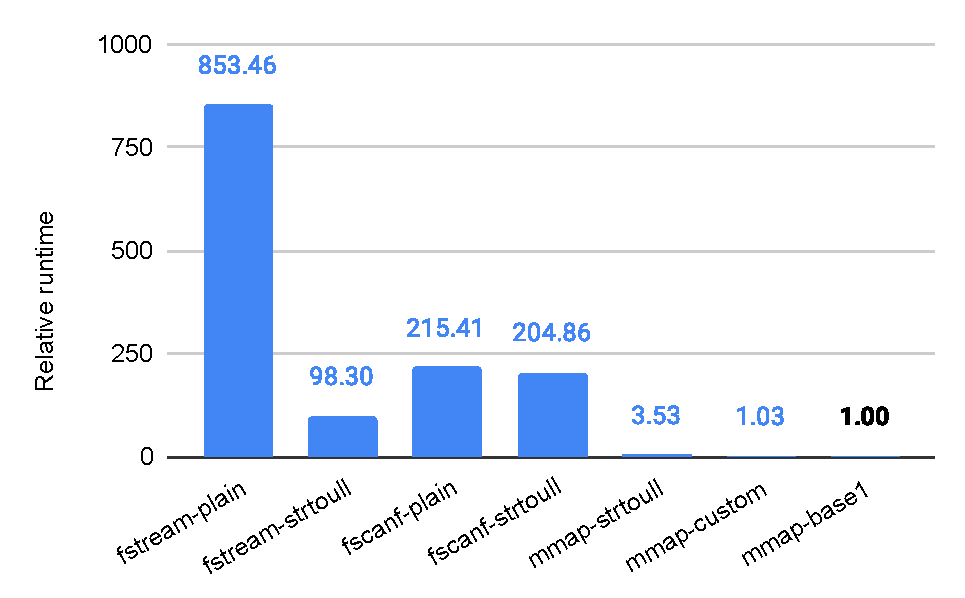
\includegraphics[width=0.99\linewidth]{out/optimize-el.pdf} \\[-2ex]
  \caption{Gini coefficient of PageRank values on 24 different graphs, comparing between PageRank values obtained with three different dead-end handling strategies: \textit{teleport from dead-ends} (\textbf{default}), \textit{self-loop dead-ends} (\textbf{loop}), and \textit{self-loop all vertices} (\textbf{loopall}).}
  \label{fig:optimize-el}
\end{figure}

\begin{figure}[hbtp]
  \centering
  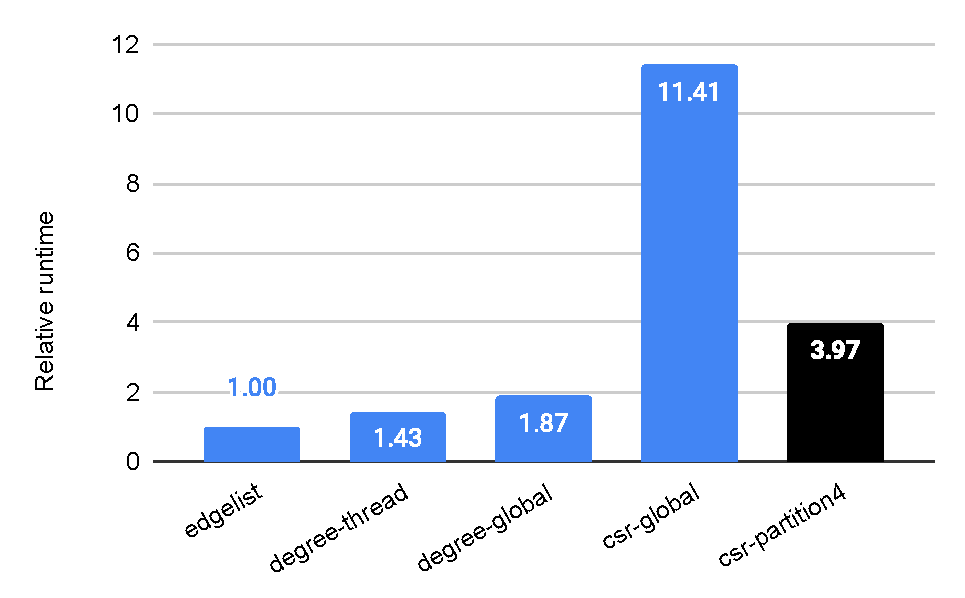
\includegraphics[width=0.99\linewidth]{out/optimize-csr.pdf} \\[-2ex]
  \caption{Gini coefficient of PageRank values on 24 different graphs, comparing between PageRank values obtained with three different dead-end handling strategies: \textit{teleport from dead-ends} (\textbf{default}), \textit{self-loop dead-ends} (\textbf{loop}), and \textit{self-loop all vertices} (\textbf{loopall}).}
  \label{fig:optimize-csr}
\end{figure}





\subsection{Converting Edgelist to CSR}

Note that we earlier obtained per-thread edgelists. We must now convert the edgelists to CSR. To do this, we first need to know the degree of each vertex. A simple solution to this is to update the degree of each vertex while loading a graph. We observe that this relsults in high contention and impact performance. In contrast, we can compute per-thread degrees. However, this a large number of additional space, and needs to be combined later to obtain global degrees. We oberve that computing degrees in partitons of 4 (using mod 4) and then combined them gives us the best perofrmance.

Now that we have the degrees, we need to combine the edges in to a CSR structure. Unfortunaltely, again using a gloval CSR has poor performance. Accordingly, we explore computing CSR in k partiones and later combining them. Our observations indicate that using 4 partitons to generate CSR and then combining them has the best operformance. Now describe the figures and the algorithm.

\begin{figure*}[hbtp]
  \centering
  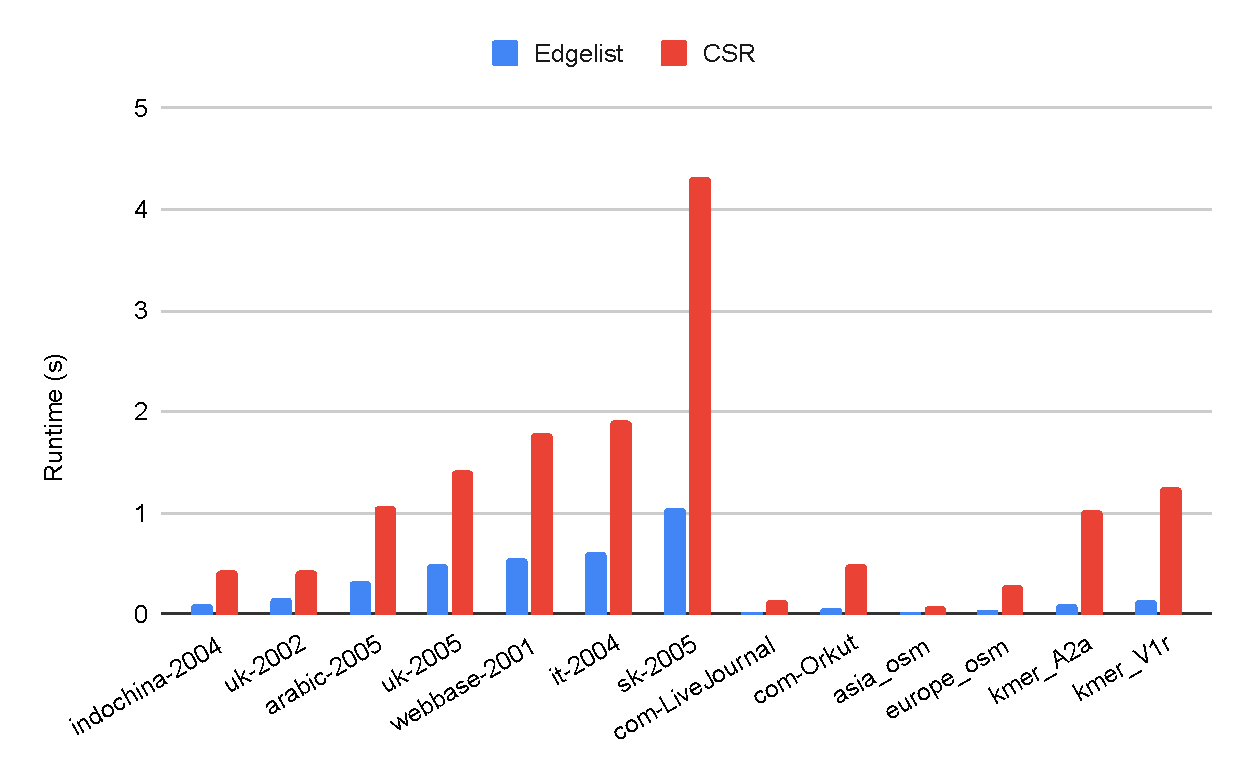
\includegraphics[width=0.68\linewidth]{out/runtime.pdf} \\[-2ex]
  \caption{Time taken by GVEL for edge-list and CSR loading on 13 different graphs.}
  \label{fig:runtime}
\end{figure*}

\begin{figure*}[hbtp]
  \centering
  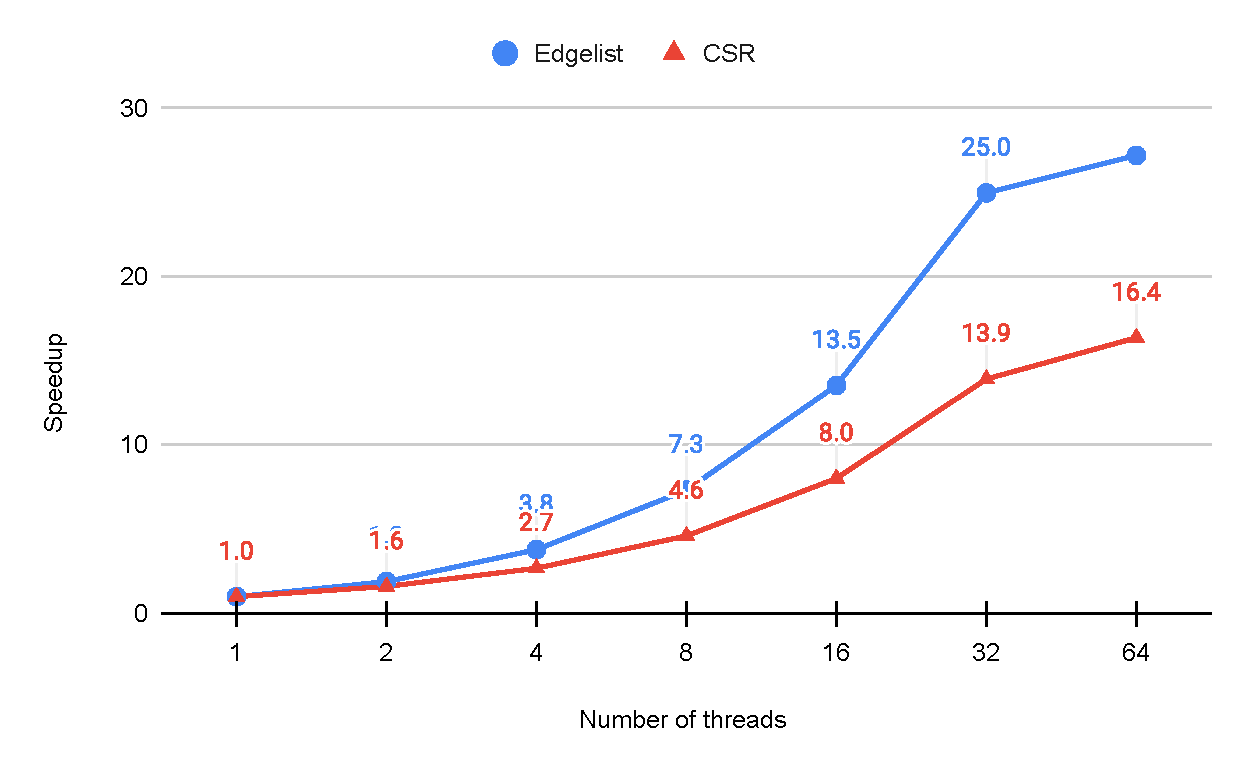
\includegraphics[width=0.68\linewidth]{out/scaling.pdf} \\[-2ex]
  \caption{Speedup of GVEL's Edgelist and CSR loading with increasing number of threads.}
  \label{fig:scaling}
\end{figure*}

\begin{figure*}[hbtp]
  \centering
  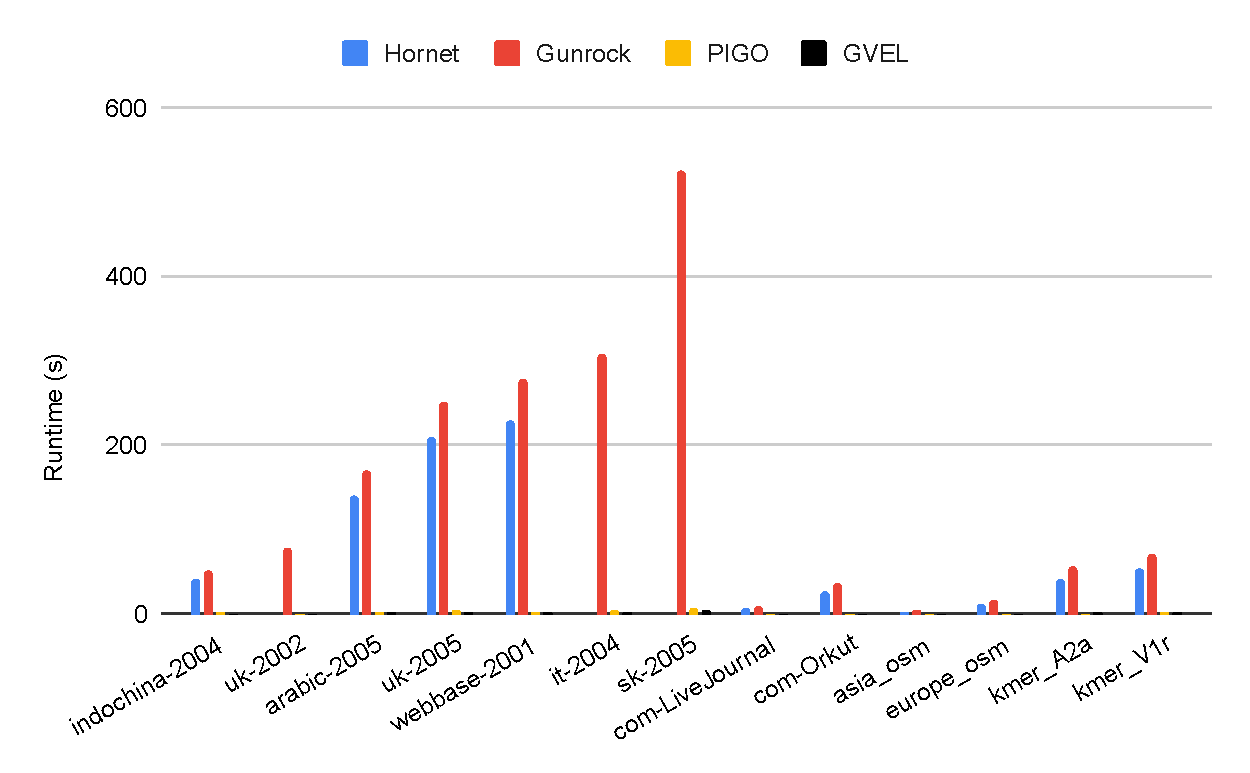
\includegraphics[width=0.68\linewidth]{out/compare-large.pdf} \\[-2ex]
  \caption{Time taken by Hornet, Gunrock, PIGO, and GVEL for reading edge-list and converting it to CSR on 13 different graphs. PIGO and GVEL are not visible on this scale - they are significantly faster than Hornet and Gunrock. The graph loading time for Hornet is not shown for \textit{uk-2002}, \textit{it-2004}, and \textit{sk-2005} graphs as it crashed while loading.}
  \label{fig:compare-large}
\end{figure*}

\begin{figure*}[hbtp]
  \centering
  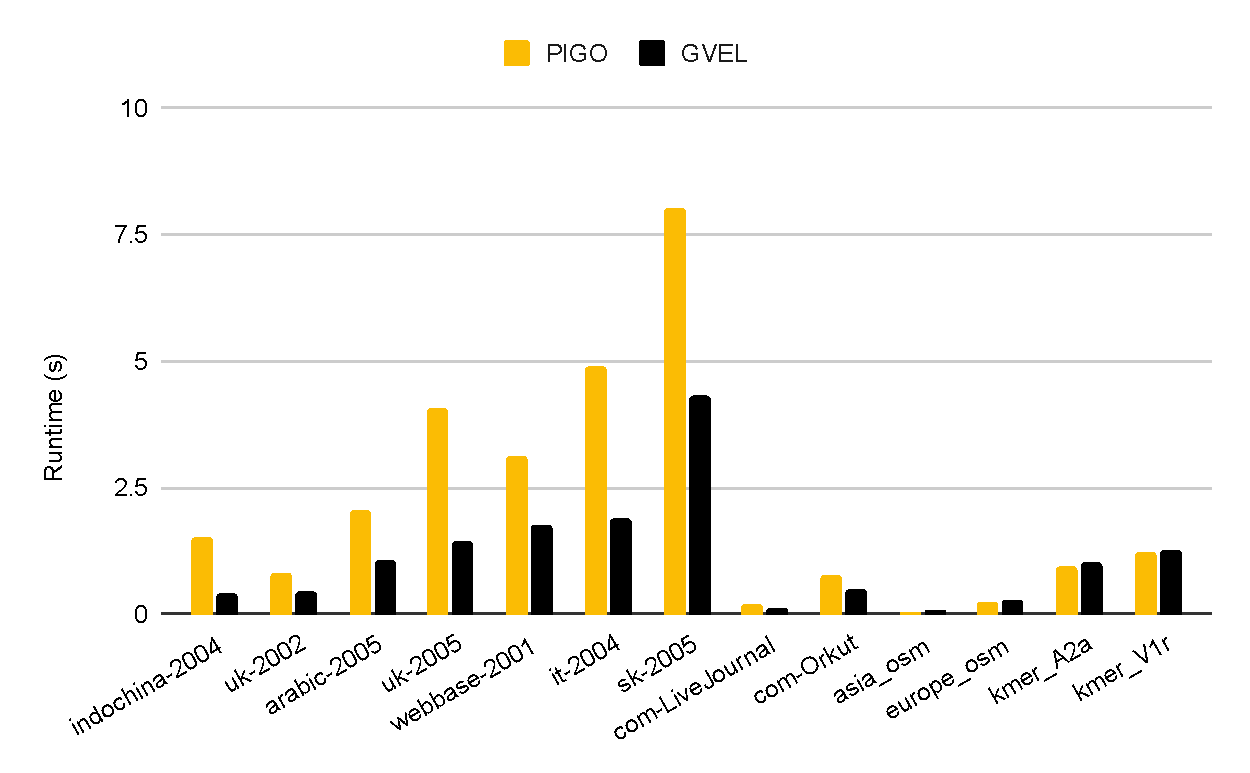
\includegraphics[width=0.68\linewidth]{out/compare-small.pdf} \\[-2ex]
  \caption{Gini coefficient of PageRank values on 24 different graphs, comparing between PageRank values obtained with three different dead-end handling strategies: \textit{teleport from dead-ends} (\textbf{default}), \textit{self-loop dead-ends} (\textbf{loop}), and \textit{self-loop all vertices} (\textbf{loopall}).}
  \label{fig:compare-small}
\end{figure*}

